\documentclass[../../FisicaTeorica.tex]{subfiles}

\begin{document}
\begin{comment}
Nella scorsa lezione abbiamo osservato la rappresentazione unitaria delle rotazioni in $\hs=L^2(\bb{R}^3,d^3x)$:
\begin{align*}
(U(\varphi, \vec{n})\psi(\vec{x})&=\psi(R^{-1}(\varphi,\vec{n}),\vec{x}); \quad U(\varphi,\vec{n})=\exp\left(i\frac{\varphi}{\hbar}\vec{L}\cdot \vec{n}\right)\\
U(2\pi,\vec{n})=\bb{I}&\Rightarrow \sigma(\vec{L}\cdot \vec{n})\subseteq \hbar \bb{Z}
\end{align*}
è questa la rappresentazione più generale delle rotazioni in \MQ? Vediamo ora che \textbf{non} è così.\\
\end{comment}
\section{Momento angolare generale}
Nei paragrafi precedenti abbiamo ricavato una rappresentazione unitaria $U(\varphi, \vec{n})$ delle rotazioni procedendo in analogia con la \MC. Ci chiediamo: è questa l'\textit{immagine più completa}, o nella stranezza della \MQ è possibile trovare altre possibilità?\\

L'unico modo di capir ciò è ripartire, in analogia alle traslazioni temporali o spaziali, dai concetti di teoria dei gruppi e delle rappresentazioni che abbiamo introdotto negli scorsi capitoli.\\

Per l'\textbf{isotropia dello spazio} sappiamo che le \textit{rotazioni} devono lasciare \textit{invariate} le \textit{probabilità di transizione}. Rappresentiamo allora le rotazioni con operatori che agiscono sugli stati, ossia in $\mathcal{PH}$, associando a ogni elemento del gruppo delle rotazioni uno di questi operatori: $G \ni g \mapsto \hat{U}(g)$.\\
Per il \textit{teorema di Wigner}, tale rappresentazione \textit{induce} una rappresentazione \textit{proiettiva} \textit{unitaria} su $\hs$, ossia possiamo vedere gli $\hat{U}(g)$ (che lavorano nello spazio proiettivo $\mathcal{PH}$ degli stati puri), come $U(g)$ che invece agiscono sul \q{normale} spazio di Hilbert $\hs$ definiti \textit{a meno di un fattore}.\\
Per rimuovere questa ambiguità potremmo usare il \textit{teorema di Bargmann}.\\
Le rotazioni sono descritte dal gruppo $SO(3)$, la cui algebra di Lie è indicata con lettere minuscole come $\mathfrak{so}(3)$. Detto un elemento $R\ni SO(3)$:
\begin{itemize}
\item $R$ è una matrice $3\times 3$, come indicato dal $(3)$.
\item $R$ è una matrice \textbf{O}rtogonale, ossia la sua inversa coincide con la trasposta: $R^T R = \bb{I}$
\item $R$ è una matrice \textbf{S}peciale, ossia con $\op{det}R=\bm{+}1$ (le matrici ortogonali, di per sé, hanno $\op{det} = \pm 1$).
\end{itemize}
Il problema è che mentre per le traslazioni temporali/spaziali partivamo da $G=(\bb{R},+)$ o $G=(\bb{R}^3,+)$, entrambi già semplicemente connessi, qui abbiamo $G=SO(3)$ che \textit{non} è semplicemente connesso!\\
Per vedere il perché, esaminiamone la sua struttura di varietà differenziale, su cui fissiamo una parametrizzazione.
\begin{figure}[H]
\centering
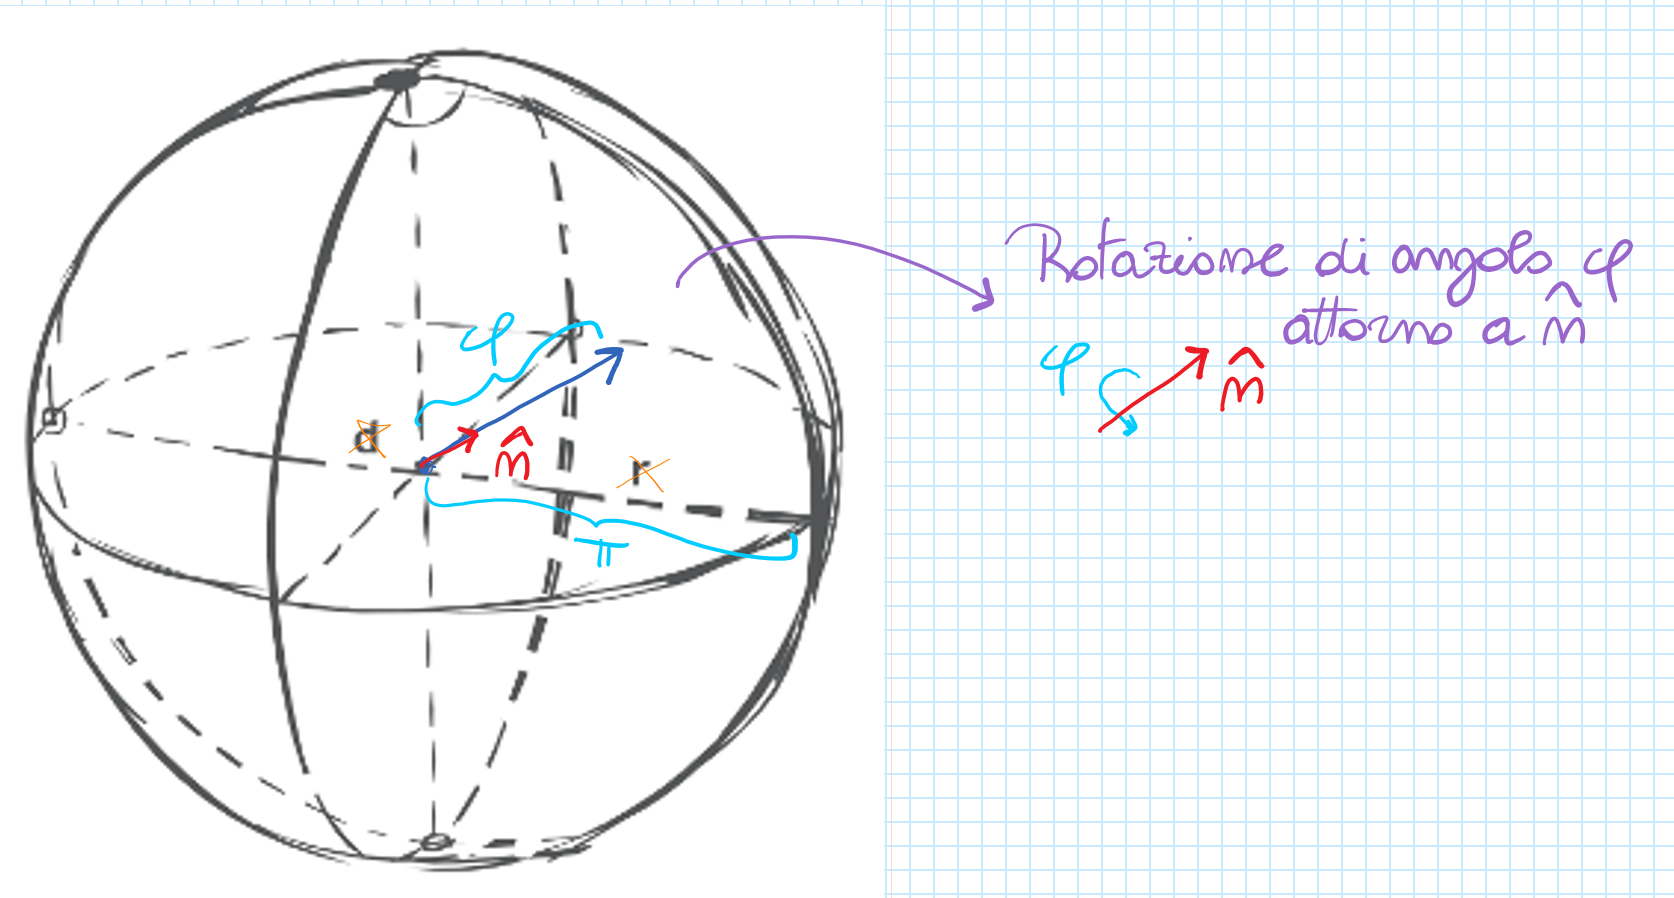
\includegraphics[scale=0.2]{Immagini/23_11/image001.png}
\caption{Parametrizzazione di $SO(3)\cong B^3/\sim$}
\end{figure}
Consideriamo la \textit{palla} $B^3$ di raggio $\pi$, ossia la \textit{sfera} 3D considerata con bordo e punti interni, che sappiamo parametrizzare, e mostriamo che è \textit{equivalente} a $SO(3)$. Detto $O$ il centro di $B^3$, un punto $P \in B^3$ definisce una direzione $OP$, che interpretiamo come l'\textit{asse} di una rotazione. La distanza di $P$ da $O$ (che sarà al più $\pi$), indica invece l'\textit{angolo di rotazione}, che sarà (convenzionalmente) in senso orario osservando \q{da $O$ verso la punta di $OP$}\footnote{Il che equivale ad applicare la \textit{regola della mano destra} puntando il pollice verso $P$ e osservando la direzione in cui si piegano le altre quattro dita.}.\\
In questo modo, usando $\varphi \in [0,\pi]$ e $\hat{n} \in \bb{R}^3$ possiamo individuare ogni punto in $B^3$, e quindi ogni rotazione in $SO(3)$.\\
In realtà c'è una correzione importante da effettuare. Notiamo che, per la nostra convenzione, ruotare di $\pi$ attorno a $\hat{n}$ produce lo stesso risultato di ruotare di $\pi$ attorno a $-\hat{n}$\footnote{Se ciò non è immediatamente chiaro, basta disegnare una freccia verso l'alto su un foglio, e ruotare il tutto di $180^\circ$ in senso antiorario: la freccia punterà in basso. Stesso risultato si ottiene riportandosi alla situazione iniziale e ruotando di $180^\circ$ in senso orario.}, dato che differiscono di una rotazione di $2\pi$ equivalente alla rotazione nulla. Ciò significa che, geometricamente, dobbiamo considerare i punti antipodali della \textit{superficie esterna} di $B^3$ come \textit{equivalenti}, visto che corrispondono a rotazioni di $\pi$ con $\hat{n}$ opposti. Se $\sim$ è tale relazione di equivalenza, indichiamo la palla con i punti antipodali identificati con $B^3/\sim$, che è finalmente \textit{isomorfa} al gruppo $SO(3)$ delle rotazioni.\\
%Inserire immagine
Possiamo allora notare che $B^3/\sim$ \textit{non} è semplicemente connessa: dato che i punti antipodali sono \textit{lo stesso punto}, un diametro di $B^3/\sim$ è un \textit{percorso chiuso}, che però non si può contrarre con continuità a un punto senza spezzarlo, dato che i suoi estremi sono vincolati a muoversi in modo \textit{speculare}  sulla superficie di $B^3$.\\
Ciò significa che il gruppo di ricoprimento di $SO(3)$ non può essere $SO(3)$ stesso:
\[
\widetilde{SO}(3) \neq SO(3)
\]
Si può dimostrare\footnote{L'idea sta nell'utilizzare i \textit{quaternioni}, che possiamo considerare come un'estensione dei numeri complessi con \q{3 unità immaginarie invece che una}, che sono in corrispondenza biunivoca con i punti di $S^3 \cong SU(2)$ - e in effetti la loro esistenza deriva proprio dal fatto che su $S^3$ si può definire una struttura di gruppo (di Lie) - cosa che per esempio non si può fare su $S^2$. Si procede dimostrando che un quaternione \textit{a meno del segno} individua una rotazione tridimensionale: perciò esiste una mappa suriettiva tra $SU(2)$ e $SO(3)$, e dato che $S^3$ è semplicemente connessa, $SU(2)$ è il ricoprimento universale di $SO(3)$. I dettagli della dimostrazione sono disponibile nella lezione $4-1$ del corso di Geometria Differenziale tenuto dal professor Francesco Bottacin} che il ricoprimento $\widetilde{SO}(3)$ è quello delle matrici $2\times 2$ \textbf{U}nitarie (complesse) a determinante $+1$ (\textbf{S}peciali), che chiamiamo $SU(2)$ (e la relativa algebra di Lie è indicata con $\mathfrak{su}(2)$). Gli elementi $T$ di $SU(2)$ hanno la forma:
\[
T =
\begin{pmatrix}
a & b\\
-b^* & a^*
\end{pmatrix} \in SU(2)
\]
Con la condizione $|a|^2 + |b|^2 = \op{det}(T) = +1$. Possiamo riscrivere tale condizione separando parti reali e immaginarie:
\[
(\op{Re} a)^2 + (\op{Im} a)^2 + (\op{Re} b)^2 + (\op{Im} b)^2 = 1
\]
Otteniamo l'equazione di una sfera\footnote{Con sfera intendiamo sempre la \textit{superficie sferica}. $S^n$ è quindi la superficie $n$-dimensionale di una sfera in $n+1$ dimensioni: $S^2$ è la superficie sferica di una normale sfera 3D, mentre $S^3$ è la \q{superficie} tridimensionale di una ipersfera, che consideriamo immersa in $\bb{R}^4$.} $S^3$ in $4$ dimensioni, che sappiamo essere semplicemente connessa (lo sono tutte le $S^n$ per $n>1$).\\

Si dimostra che ogni punto di $S^3$ parametrizzata \textit{cartesianamente} con $(\op{Re}a, \op{Im}a, \op{Re}B, \op{Im}b)$ corrisponde, \textit{a meno del segno}, a un'unica rotazione in $SO(3)$). Matematicamente, si ha una mappa suriettiva $\tilde{g}: SU(2) \cong \tilde{SO}(3) \to SO(3)$ (che nello specifico è un \textit{ricoprimento a due fogli}) data da:
\[
\pm (\op{Re}a, \op{Im}a, \op{Re}b, \op{Im}b) \mapsto \tilde{g}(\op{Re}a, \op{Im}a, \op{Re}b, \op{Im}b)
\]

Geometricamente, $\tilde{g}$ collega punti antipodali su $S^3$ alla stessa rotazione in $SO(3)$.\\

Cerchiamo di dare un'intuizione \textit{pittoresca} della situazione. Spostiamoci in dimensione inferiore, e partiamo da $B^2$, ossia da un \textit{cerchio} (inteso come circonferenza + punti interni), i cui punti rappresentano le \textit{trasformazioni} che stiamo esaminando\footnote{\textit{Approfondimento}: In realtà, i punti di $B^2$ non rappresentano, come ci si potrebbe aspettare, le rotazioni in $2D$, che sono invece individuate dai punti di $B^1$ - con antipodi identificati - ossia dalla circonferenza unitaria $S^1 \cong U(1)$. In effetti il ricoprimento $S^2$, inteso come varietà, è \textit{incompatibile} con una struttura di gruppo.}.
Come prima, identifichiamo gli antipodi di $B^2$, dato che nella nostra analogia corrisponderebbero alle \textit{stesse trasformazioni}. Abbiamo quindi che $B^2$ non è semplicemente connesso (un diametro di $B^2$ è un percorso chiuso che non si può contrarre a un punto con continuità).\\
Vogliamo trovare un'altra varietà $\tilde{G}$, che sia semplicemente connessa, tale che esista una mappa suriettiva $\tilde{g}:\tilde{G}\to B^2$, ossia per cui ogni punto di $B^2$ abbia \textit{almeno una controimmagine} in $\tilde{G}$.\\
Proviamo con $S^2$ (visto che nel caso a dimensione maggiore abbiamo usato $S^3$), che è la superficie di una sfera tridimensionale - ed è semplicemente connessa.\\
Allora, pittorescamente, si consideri una sfera unitaria centrata all'origine di un piano cartesiano, e il piano $\hat{x}\hat{y}$ che la \textit{taglia} a metà. $\tilde{g}$ si può interpretare come la \textit{proiezione} dei punti della sfera sul piano. In particolare, notiamo che ogni punto del cerchio unitario $B^2$ sul piano $\hat{x}\hat{y}$ si ottiene dalla proiezione di almeno un punto di $S^2$.\\
Graficamente, notiamo che ci sono sempre due punti di $S^2$ che \textit{si proiettano} nello stesso punto di $B^2$: uno \q{dall'alto} e uno \q{dal basso}. In realtà dobbiamo considerare che i punti di $S^2$ all'intersezione con il piano $z=0$ sono \textit{proiettati su se stessi}, ma dobbiamo ricordarci che in $B^2$ abbiamo identificato i punti antipodali, e quindi anche qui è come avere \textit{due proiezioni} per lo stesso punto.
\begin{figure}[H]
\centering
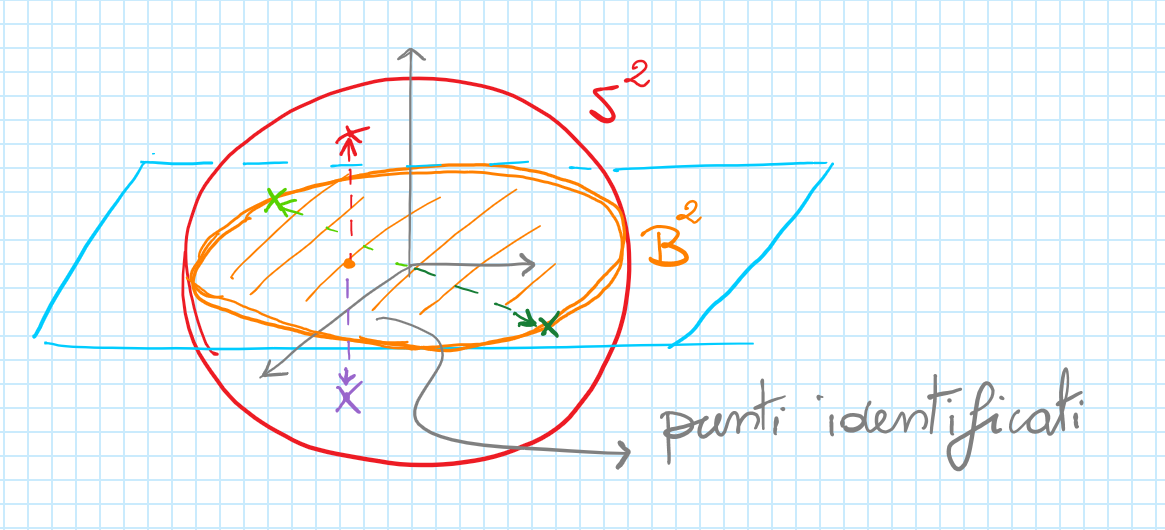
\includegraphics[scale=0.2]{Immagini/23_11/image002.png}
\caption{Ogni punto di $B^2/\sim$ è \textit{originato} dalla proiezione di esattamente \textit{due} punti di $S^2$}
\end{figure}
Possiamo allora comprendere la definizione di $\tilde{g}$ come \textit{a meno del segno}: così facendo stiamo \q{eliminando tutti i doppioni}. Visivamente, ciò significa considerare un solo emisfero (per esempio $S^2_+$), con \textit{mezzo bordo} (dato che anche per i punti su $z=0$ vi sono \textit{due proiezioni}).\\
Notiamo altre due cose:
\begin{itemize}
\item Un diametro di $B^2$, che è il cammino chiuso e incomprimibile che prima dava problemi, risulta come la proiezione di una \textit{circonferenza massimale} su $S^2$, che stavolta è comprimibile a un punto.
\item Una rotazione di $2\pi$ corrispondeva in $B^3$ (e quindi anche in $B^2$, per analogia) a passare da un punto sul \textit{bordo} al suo punto antipodale (e infatti i due coincidono su $B^2$). La stessa cosa non si ha più su $S^2$, dato che tale punto è proiezione di \textit{due punti} non coincidenti. Solo ripetendo un'ulteriore rotazione di $2\pi$ anche in $S^2$ i due punti coincideranno.\\
Stessa cosa si può dimostrare, perdendo però ogni visualizzazione, nel caso a dimensione $3$ che ci interessa, ossia per $SO(3)\cong B^3/\sim$ e $S^3 \cong SU(2) \cong \widetilde{SO}(3)$.\\
Ciò ha conseguenze fondamentali: se decidiamo di utilizzare una rappresentazione unitaria senza ambiguità di fasi (e quindi \textit{non proiettiva}) tramite il teorema di Bargmann, dovremo spostarci sul gruppo di ricoprimento, che \textit{non} segue le stesse \q{regole} del gruppo di partenza: su $B^3/\sim$ la rotazione di $2\pi$ è nulla, su $S^3$ è quella di $4\pi$ a essere nulla.
\end{itemize}
\begin{figure}[H]
\centering
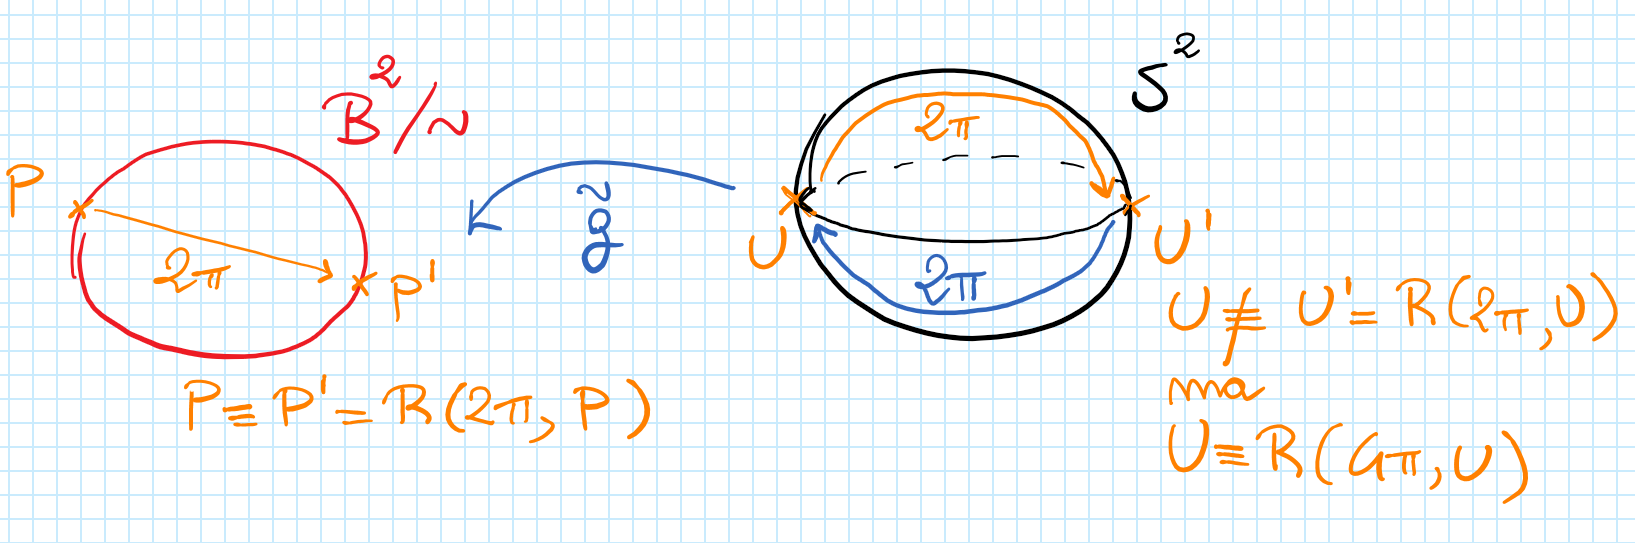
\includegraphics[scale=0.2]{Immagini/23_11/image004.png}
\caption{Una rotazione di $2\pi$ su $B^2/\sim$ \q{non sposta il punto} $P$, dato che $P$ e $P'$ sono identificati da $\sim$, ma lo sposta sul ricoprimento $S^2$, dove partendo da $U$ si ritorna a $U$ solo dopo una rotazione di $4\pi$}
\end{figure}

Applicando allora il teorema di Bargmann, troviamo che una una rappresentazione unitaria in $\hs$ di una rotazione $\tilde{R} \in SU(2)$ sul gruppo di ricoprimento universale di $SO(3)$ sarà una certa $\tilde{U}(\varphi,\vec{n})$, che per teorema di Stone si ottiene dalla mappa esponenziale applicata ad un elemento (o meglio ad una sua rappresentazione) dell'algebra di Lie $\mathfrak{su}(2)$. Detta $\vec{J}$ una rappresentazione in un insieme (denso) di $\hs$ dei generatori (base) dell'algebra di Lie di $SU(2)$ si ha:
\[
\tilde{U}(\varphi,\vec{n}) = \exp\left(-i\frac{\varphi}{\hbar}\vec{n}\cdot \vec{J}\right)
\]
Come abbiamo visto nella teoria, l'algebra di Lie dipende unicamente dalle caratteristiche \textit{locali} del gruppo da cui deriva. Poiché un gruppo e ricoprimento universale sono \textit{localmente identificati}, da $\tilde{SO}(3) \cong SU(2)$, si ha $\mathfrak{su}(2) \cong \mathfrak{so}(3)$. In particolare, l'algebra di $\vec{J}$ è la stessa dei generatori delle rotazioni, quindi la stessa di $\vec{L}$. In pratica, possiamo riutilizzare per $\vec{J}$ i commutatori già calcolati per $\vec{L}$:
\begin{equation}
[J_i, J_j] = i\hbar \epsilon_{ijk}J_k
\label{eqn:condizione_j}
\end{equation}
Poiché tuttavia una rotazione di $2\pi$ in $\tilde{SO}(3)$ non è equivalente alla rotazione nulla, per $\vec{J}$ \textbf{non} abbiamo più la condizione sugli autovalori  $\sigma(\vec{J}\cdot \vec{n}) \subseteq \hbar \bb{Z}$, .\\
$\vec{J}$ sarà chiamato \textbf{momento angolare} se soddisfa (\ref{eqn:condizione_j}) e $\vec{L}=\vec{X}\land \vec{P}$ verrà detto \textbf{momento angolare orbitale}.\\

Da (\ref{eqn:condizione_j}) sappiamo che, come ricavato per $\vec{L}$, $\vec{J}^{\,2}, J_3$ sono compatibili, e quindi possiamo cercare \textit{autovettori comuni}.\\
Una procedura efficiente per far ciò consiste nel notare che, trovato un autovettore comune, possiamo \q{costruire} tutti gli altri, tramite l'applicazione di opportuni operatori che \q{alzano} e \q{abbassano} gli autovalori.\\

Definiamo allora $J_{\pm} \equiv J_1 \pm i J_2$, ove $J_- = (J_+)^\dag$. Ricaviamone subito le relazioni di commutazione. Ricordando (\ref{eqn:condizione_j}) e sfruttando la bilinearità del commutatore si ha:
\begin{align}\nonumber
[J_3, J_{\pm}] &= [J_3, J_1 \pm i J_2] = i\hbar (\overbrace{\epsilon_{312}}^{1} J_2 \pm i\overbrace{ \epsilon_{321}}^{-1}J_1) =\\
&=i\hbar (J_2 \mp iJ_1) = \hbar (\pm i J_2 + J_1) = \pm \hbar(J_1 \pm i J_2) = \pm \hbar J_\pm
\label{eqn:commutazione_Jpm}
\\
[J_+, J_-] &= [J_1 + iJ_2, J_1 - iJ_2]=i[J_2, J_1]-i[J_1,J_2]=\\
&= i(i\hbar\underbrace{\epsilon_{123}}_{1}J_3) -i(i\hbar\underbrace{ \epsilon_{213}}_{-1}J_3)=
2\hbar J_3 \nonumber
\end{align}

Sia ora $\ket{\lambda,m}$ un autovettore comune di $\vec{J}^2$ e $J_3$, espresso in notazione di Dirac, di autovalore $\hbar^2 \lambda$ per $\vec{J}^2$ e $\hbar m$ per $J_3$, ossia tale che:
\begin{align}
\vec{J}^2 \ket{\lambda,m} &= \hbar^2 \lambda \ket{\lambda,m}
\label{eqn:autovalJquadro}
\\
J_3 \ket{\lambda,m} &=\hbar m \ket{\lambda,m} 
\label{eqn:autovalJ3}
\end{align}
In tal modo abbiamo \q{adimensionalizzato} la notazione dell'autovettore, dato che $\lambda, m \in \bb{R}$.\\
Mostriamo ora che $J_+$ e $J_-$, se applicati a $J_3$ rispettivamente ne \q{alzano} e \q{abbassano} l'autovalore $\hbar m$, e quindi ci permettono di trovare gli altri autovalori. Infatti, applicandoli a $J_3$ otteniamo:
\begin{align}\nonumber
J_3 \hlc{Yellow}{J_{\pm} \ket{\lambda,m}} &= ([J_3,J_\pm]+J_\pm J_3)\ket{\lambda,m} \underset{(\ref{eqn:commutazione_Jpm})}{=}
J_\pm (J_3 \pm \hbar) \ket{\lambda, m} = \\
&\underset{(\ref{eqn:autovalJ3})}{=} J_\pm (m\hbar \pm \hbar) \ket{\lambda,m} = \hbar(m\pm 1)\hlc{Yellow}{ J_{\pm}\ket{\lambda,m}} \label{eqn:autovalore_aumentato}
\end{align}
ovvero $J_\pm\ket{\lambda,m}$ è autovettore di $J_3$ con autovalore $\hbar(m\pm 1)$ (solo se $\ket{\lambda,m}$ è autovettore e $J_\pm \ket{\lambda,m}\neq 0$).\\ %Non potrebbe "uscire da L^2"?

Il passo successivo sta nel riscrivere $\vec{J}^2$ utilizzando gli operatori $J_\pm$ e $J_3$. Partiamo esaminando un classico risultato dell'algebra alla luce di operatori che non commutano. La scomposizione:
\begin{align*}
a^2 + b^2 = (a-ib)(a+ib)
\end{align*}
deve essere adattata per la non commutatività. Infatti, se calcoliamo il termine a destra per $A$ e $B$ che non commutano:
\begin{align*}
(A-iB)(A+iB)&=A^2 +iAB - iBA +B^2=A^2 +B^2 +i[A,B]\\
&\Rightarrow A^2+B^2 = (A-iB)(A+iB)-i[A,B]
\end{align*}
Possiamo applicare ciò al nostro caso, dato che $\vec{J}^2$ è una somma di quadrati:
\begin{align}\nonumber
\vec{J}^{\,2}&= J_1^2 + J_2^2 + J_3^2 = \hlc{Yellow}{(J_1 \mp i J_2)(J_1 \pm i J_2)} \hlc{SkyBlue}{\mp i [J_1,J_2]}+J_3^2 =\\
&\underset{(\ref{eqn:commutazione_Jpm})}{=} \hlc{Yellow}{J_\mp J_\pm} \hlc{SkyBlue}{\pm \hbar J_3} + J_3^2 \label{eqn:Jquadro}
\end{align}
Riarrangiando, troviamo che:
\begin{align}
J_\mp J_\pm = \vec{J}^2 \mp \hbar J_3 - J_3^2
\label{eqn:jpjm}
\end{align}

Ciò che abbiamo appena calcolato ci è utile per esaminare il \textit{modulo} degli autovettori di $J_3$ \q{aumentati} o \q{abbassati} rispettivamente da $J_+$ e $J_-$.
\begin{align}\nonumber
0 &\leq \norm{J_+ \ket{\lambda,m}}^2 = \bra{\lambda, m} J_+^\dag J_+ \ket{\lambda, m} = \bra{\lambda, m}J_- J_+ \ket{\lambda, m} =\\
&\underset{(\ref{eqn:jpjm})}{=} \bra{\lambda, m} \vec{J}^{\,2} - \hbar J_3 - J_3^2 \ket{\lambda, m}= \hbar^2 (\lambda - m - m^2) = \hbar^2(\lambda-m(m+1))
\label{eqn:piu1}\\
0 &\leq \norm{J_- \ket{\lambda,m}}^2 = \bra{\lambda,m}J_+ J_- \ket{\lambda,m} = \nonumber \\
&\underset{(\ref{eqn:jpjm})}{=} \bra{\lambda,m}\vec{J}^{\,2} + \hbar J_3 - J_3^2 \ket{\lambda,m} = \hbar^2 (\lambda-m(m-1)) \label{eqn:meno1}
\end{align}
Poiché $\lambda$ è fissato, notiamo allora che il modulo degli autovettori di autovalore maggiore o minore rispettivamente sale o scende. Ci aspettiamo che ciò non possa andare avanti all'infinito, dato che il modulo non può scendere sotto zero, né salire infinitamente. In effetti, nei prossimi passaggi mostreremo che esistono un $m_{\min}$ e un $m_{\max}$.\\

Partiamo sommando le disuguaglianze (\ref{eqn:piu1}) e (\ref{eqn:meno1}): 
\begin{align*}
\lambda - m^2 \geq 0 \Rightarrow \lambda \geq m^2 \geq 0 \Rightarrow  \exists \sqrt{\lambda}
\end{align*}
E quindi calcolando la radice quadrata di ambo i membri giungiamo a:
\begin{equation}
|m| \leq \sqrt{\lambda}
\label{eqn:condizione_m}
\end{equation}

Sappiamo da (\ref{eqn:autovalore_aumentato}) che, applicando $J_+$ e $J_-$ a $\ket{\lambda,m}$, possiamo alzare o abbassare arbitrariamente l'autovalore di $J_3$ senza modificare $\lambda$, ma ciò avviene solo a meno che l'applicazione di $J_+$ o $J_-$ non dia il vettore nullo.\\

Perché allora sia la (\ref{eqn:autovalore_aumentato}) che la (\ref{eqn:condizione_m}) siano contemporaneamente vere, si ha che fissato $\lambda$ deve esistere un $m_{\min}$ tale che $J_- \ket{\lambda, m_{min}}=0$, e simmetricamente anche un $m_{\max}$, per cui $J_{max}\ket{\lambda, m_{max}} = 0$, ossia due autovalori che \q{interrompono la catena} e oltre i quali non si può più né scendere né salire\footnote{Il riferimento è voluto.}.\\

Cosa succede applicando $\vec{J}^2$ agli autoket di $m$ max o min? Vediamolo:\begin{align*}
\hlc{Yellow}{\vec{J}^{\,2}} \ket{\lambda, m_{max}} &= \hbar^2 \lambda \ket{\lambda, m_{max}} \underset{(\ref{eqn:Jquadro})}{=} \hlc{Yellow}{(\underbrace{J_- J_+}_{0} + \hbar J_3 + J_3^2)} \ket{\lambda, m_{max}} =
\\&= \hbar^2(m_{max}+m_{max}^2)\ket{\lambda, m_{max}} \Rightarrow \lambda = m_{max} + m^2_{max}\\
\hlc{SkyBlue}{\vec{J}^{\,2}}\ket{\lambda, m_{min}} &= \hbar^2 \lambda \ket{\lambda, m_{min}} \underset{(\ref{eqn:Jquadro})}{=
}\hlc{SkyBlue}{(\underbrace{J_+ J_-}_{0} - \hbar J_3 + J_3^2)} \ket{\lambda, m_{min}} =\\&= (-m_{min}+m_{min}^2) \ket{\lambda, m_{min}} \Rightarrow \lambda = -m_{min} + m_{min}^2
\end{align*}
dato che $J_+$ applicato all'autoket con $m_{max}$ non può alzarlo ulteriormente, e quindi ritorna il vettore nullo, e stessa cosa per $J_-$ applicato all'autoket con $m_{min}$.

Dato che in tutto ciò $\lambda$ non cambia, possiamo scrivere:
\begin{align*}
\lambda = m_{max} + m_{max}^2 = -m_{min} + m_{min}^2
\end{align*}
che è verificata se $m_{max}=-m_{min} \equiv j > 0$, da cui $\lambda=j(j+1)$.\\
Poiché applicando $N+1$ volte $J_-$ all'autoket $\ket{j,j=m_{max}}$ dobbiamo ottenere $0$ per un qualche $N$ abbiamo che:
\[
\underbrace{J_-^N \ket{j,j}}_{\propto \ket{j, j-N}} \propto \ket{j, m_{min} =-j} \Rightarrow  j-N = -j \Rightarrow  2j = N \in \bb{N} \Rightarrow  j \in \frac{\bb{N}}{2} \Rightarrow  m \in \frac{\bb{Z}}{2}
\]
L'idea è che, come abbiamo visto, i valori possibili per $m$ vanno da $m_{\min}=-j$ a $m_{\max}=+j$, sono a distanza unitaria (a meno di un $\hbar$) uno dall'altro e sono in \textit{numero finito}. Possiamo pensarli come una successione di $2N+1$ \textit{puntini} \q{centrata} attorno allo $0$ della retta reale. Se $N$ è pari, avremo un autovalore a $0$ e gli altri a $\pm i$, ma se $N$ è dispari allora gli autovalori saranno per forza del tipo $\pm i/2$.\\

%[IMMAGINE] disegnetto degli autovalori come puntini equidistanziati sulla retta reale, nel caso siano in numero pari o dispari

Esplicitamente, fissato allora $j \in \bb{N}/2$ i possibili valori di $m$ sono:
\[
\{j, j-1, j-2, \dots, -j+1, -j\}
\]
che coprono $2j+1$ possibilità.\\
%[CFR Pag. 192 Sakurai]
Se imponiamo a $\ket{j,m}$ di avere norma $1$: %[TO DO] Sistemare qua
\begin{align*}
J_\pm \ket{j,m} &= c_\pm (j,m) \ket{j, m\pm 1}\\
\norm{J_+ \ket{j,m}}^2&=|c_\pm (j,m)|^2
\end{align*}

Da cui:
\begin{align*}
\norm{J_\pm \ket{\lambda,m}}^2=\hbar^2(\lambda-m(m\pm 1)) =\hbar^2(j(j+1)-m(m\pm 1)) = |c_{\pm}(j,m)|^2
\end{align*}
Con una scelta opportuna di fase possiamo infine scrivere:
\[
J_\pm \ket{j,m}=\sqrt{j(j+1)-m(m\pm 1)} \ket{j, m\pm 1}
\]
Abbiamo allora dimostrato che, se esiste un autoket $\ket{j,j}$ \q{da cui partire} vale: 
\[
\sigma_P(\vec{J}^{\,2}; J_3) = \{\underbrace{ \hbar^2(j(j+1)), j\in \frac{\bb{N}}{2}}_{\sigma(\vec{J}^{\,2})}; \underbrace{\hbar m , m = -j, -j+1, \dots, j}_{\sigma(J_3)} \}
\]
Notiamo che lo spettro è puramente \textbf{discreto}, dato che nei ragionamenti abbiamo usato delle \textit{norme}, e quindi gli autostati devono essere normalizzabili. Inoltre partendo da un punto qualsiasi e \textit{costruendo} gli altri autovalori otteniamo \textit{tutti} gli autovalori, dato che, come vedremo, i loro autovettori formano una base di $L^2$.\\

Il vero aspetto importante, tuttavia, è dato dal fatto che per ricavare tale spettro comune siamo partiti \textit{unicamente} dalle relazioni di commutazione, e in particolare da:
\[
[J_i, J_k] = i\hbar \epsilon_{ijk} J_k
\]
Ciò significa che le conclusioni raggiunte valgono anche per tutte le altre osservabili che soddisfano tali relazioni! 

\end{document}

